\documentclass[12pt,a4paper]{article}
\title{IMPs Chapitre 3}
\date{\today}
\author{Tewann Beauchard}
\usepackage[utf8]{inputenc}
\usepackage{amsmath}
\usepackage{amsfonts}
\usepackage{amssymb}
\usepackage{mathpazo}
\usepackage[T1]{fontenc}
\usepackage[french]{babel}
\usepackage{graphicx} 

\begin{document}

\begin{center}
\section*{Objectifs du stage}
\vspace*{1cm}
Tewann Beauchard \\
\vspace*{1cm}
May, 2022
\end{center}
\vspace*{1cm}

Lecture du livre INTEGRATED POPULATION MODELS, Theory and Ecological Applications with R and JAGS écrit par Michael Schaub et Marc Kéry (Chapitres 3, 5 et 6): \\
- Répétabilité des résultats\\
- Reproduction des boxplots des moyennes et des écart-type des posterior (page 250 du livre) en partant de deux hypothèses : (1)Estimation des différents paramètres démographiques (productivité,taux de croissance et de survie...) à partir des données de comptage sans dissocier les classes d'âges au sein de ces dernières ($n(t)$).(2)Estimation des différents paramètres démographiques (productivité,taux de croissance et de survie...) à partir des données de comptage en dissociant les classes d'âges au sein de ces dernières ($n_{a}(t)$ et $n_{j}(t)$).\\
\section{Écriture des équations des différents modèles composants un IPM}
En ayant pour point de départ la vraisemblance jointe d'un IPM, correspondant à la vraisemblance du modèle "ipm1.txt" (code $IPMboxplot.Rmd$) :\\
\begin{equation}
\begin{aligned}
L_{IPM}(N, s_{j}, s_{a}, p, f_{1}, f_{a}, \sigma^{2}|\textit{m},J,C)= \\
L_{I}(N_{1})\times L_{S}(N_{2,....T}, s_{j}, s_{a}, f_{1}, f_{a})\times L_{O}(N,\sigma^{2}|C)\times L_{CJS}(s_{j}, s_{a}, p|\textit{m})\times L_{p}(f_{1}, f_{a}|J)
\end{aligned}
\end{equation}
Il est facile de la décliner pour l'appliquer aux trois autres modèles présents dans le code. Pour le cas du modèle "ipm2.txt", sans la productivité (soit la régression de Poisson), nous avons : 
\begin{equation}
\begin{aligned}
L_{IPM}(N, s_{j}, s_{a}, p, f_{1}, f_{a}, \sigma^{2}|\textit{m},C)= \\
L_{I}(N_{1})\times L_{S}(N_{2,....T}, s_{j}, s_{a}, f_{1}, f_{a})\times L_{O}(N,\sigma^{2}|C)\times L_{CJS}(s_{j}, s_{a}, p|\textit{m})
\end{aligned}
\end{equation}
Si nous portons maintenant notre attention sur le modèle "imp3.txt", c'est-à-dire sans la partie capture-marquage-recapture (soit le modèle CJS), nous avons :
\begin{equation}
\begin{aligned}
L_{IPM}(N, s_{j}, s_{a}, f_{1}, f_{a}, \sigma^{2}|J,C)= \\
L_{I}(N_{1})\times L_{S}(N_{2,....T}, s_{j}, s_{a}, f_{1}, f_{a})\times L_{O}(N,\sigma^{2}|C)\times L_{p}(f_{1}, f_{a}|J)
\end{aligned}
\end{equation}
Finalement, il ne reste plus que le modèle "ipm4.txt", correspondant uniquement aux données de comptage (soit uniquement le modèle espace d'état et la partie observation), pour lequel nous avons : 
\begin{equation}
\begin{aligned}
L_{IPM}(N, s_{j}, s_{a}, f_{1}, f_{a}, \sigma^{2}|C)= \\
L_{I}(N_{1})\times L_{S}(N_{2,....T}, s_{j}, s_{a}, f_{1}, f_{a})\times L_{O}(N,\sigma^{2}|C)
\end{aligned}
\end{equation}

Il est important de noter qu'à ce stade, ce dernier modèle ne correspond techniquement pas à un IPM.\\
Dès lors que ces vraisemblances jointes sont écrites, nous pouvons nous intéresser individuellement à l'écriture des modèles composants un IPM (toujours dans le code $IPMboxplot.Rmd$). En effet, pour le modèle concernant l'estimation des données de comptage, soit le modèle espace d'état, nous avons l'équation suivante : 
\begin{equation}
N_{t+1}=N_{t}s_{a}+f\dfrac{1}{2}s_{j}N_t
\end{equation}
Dès lors les vraisemblances jointes et les équations individuelles des modèles écrites,nous pouvons nous tourner vers le vrai but de cette étude. Un étude où nous simulons et où nous estimons ces modèles avec des comptages à la fois sur les juvéniles et sur les adultes.
Ce qui donnerait, pour le modèle espace d'état : 
\begin{equation}
\begin{aligned}
   N_{j, t+1} = (1-\gamma)N_{j, t}s_{j}+0.5fN_{a, t}\\
   N_{a, t+1} = N_{a, t}s_{a}+ \gamma N_{s, t}s_j
\end{aligned}
\end{equation}
Avec $\gamma$ correspondant à une constante de transition d'un stade à un autre.\\

Maintenant, nous portons notre attention sur les boxplots d'intérêts présentant les différents paramètres démographiques et leurs écart-types.  Plus particulièrement, nous nous concentrons sur la comparaison entre ceux issus de modèles où il n'y a aucune dissociation des stades juvéniles et adultes pour les données de comptage et ceux où justement il y a cette dissociation. Pour débuter, nous effectuons 50 simulations sur les différents modèles :

\begin{figure}[!t]
\includegraphics[width=17cm]{50sim_Counts.png}
\caption{Boxplots des moyennes et des écart-types (SD) à posteriori de la survie des juvéniles ($s_j$) et des adultes ($s_a$), de la productivité($f$), et des taux de croissance de la population ($\lambda$) depuis quatre modèles démographiques différents utilisant différentes combinaisons de jeux de données : (1) IPM avec la capture-recapture, la productivité, et les données de comptage de la population ($CR \& P \& C$) ; (2) IPM avec la capture-recapture et les données de comptage de la population ($CR \& C$) ; (3)IPM avec la productivité et les données de comptage de la population ($P \& C$) ; et finalement (4) Un modèle démographique espace d'état avec les données de comptage de la population ($C$). Ces boxplots sont les résumés des moyennes à posteriori sur 50 simulations. La ligne horizontale en pointillés présente sur les trois premiers graphiques correspond aux valeurs du paramètre utilisées pour la simulation de données.}
\end{figure}
\begin{figure}[!t]
\includegraphics[width=17cm]{50sim_CountsJAD.png}
\caption{Boxplots des moyennes et des écart-types (SD) à posteriori de la survie des juvéniles ($s_j$) et des adultes ($s_a$), de la productivité($f$), et des taux de croissance de la population ($\lambda$) depuis quatre modèles démographiques différents utilisant différentes combinaisons de jeux de données : (1) IPM avec la capture-recapture, la productivité, et les données de comptage de la population dissociant la classe d'âge juvénile de celle des adultes ($CR \& P \& C$) ; (2) IPM avec la capture-recapture et les données de comptage de la population ($CR \& C$) ; (3)IPM avec la productivité et les données de comptage de la population dissociant la classe d'âge juvénile de celle des adultes ($P \& C$) ; et finalement (4) Un modèle démographique espace d'état avec les données de comptage de la population dissociant la classe d'âge juvénile de celle des adultes ($C$). Ces boxplots sont les résumés des moyennes à posteriori sur 50 simulations. La ligne horizontale en pointillés présente sur les trois premiers graphiques correspond aux valeurs du paramètre utilisées pour la simulation de données.}
\end{figure}

Nous pouvons observer que la différence la plus marquante s'opère sur le modèle démographique $P \& C$. En effet, dissocier les classes d'âges pour ce modèle permet une meilleure estimation de la survie des juvéniles (en réduisant la valeur de la SD) et une estimation plus proche de la valeur utilisée pour la simulation, notamment pour la productivité. A contrario, l'estimation est moins précise pour la survie des adultes avec une SD beaucoup plus étendue.



\begin{figure}[!t]
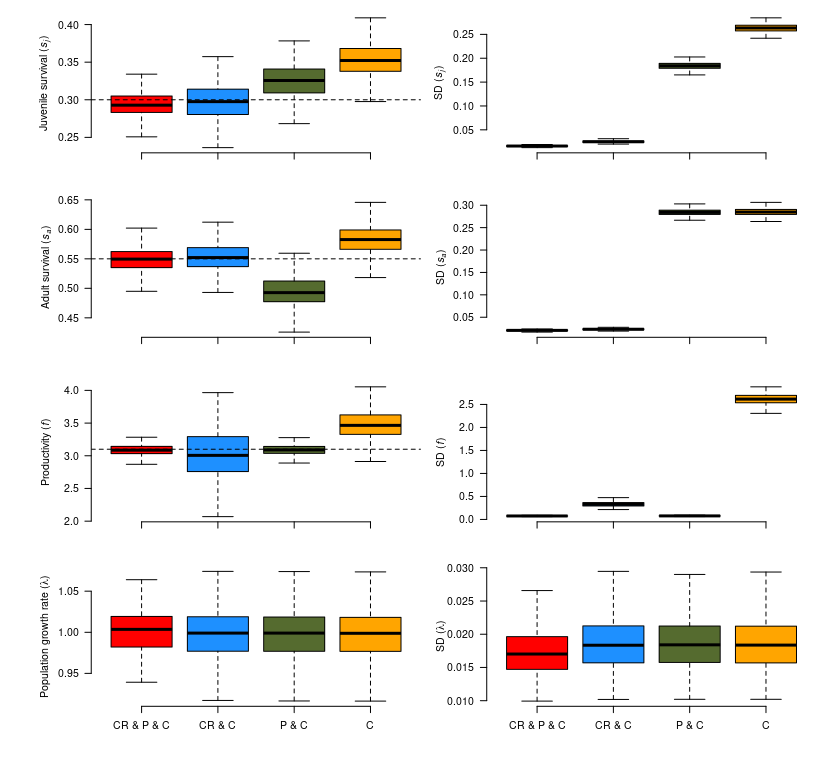
\includegraphics[width=17cm]{500sim_Counts_28062022.png}
\caption{Boxplots des moyennes et des écart-types (SD) à posteriori de la survie des juvéniles ($s_j$) et des adultes ($s_a$), de la productivité($f$), et des taux de croissance de la population ($\lambda$) depuis quatre modèles démographiques différents utilisant différentes combinaisons de jeux de données : (1) IPM avec la capture-recapture, la productivité, et les données de comptage de la population ($CR \& P \& C$) ; (2) IPM avec la capture-recapture et les données de comptage de la population ($CR \& C$) ; (3)IPM avec la productivité et les données de comptage de la population ($P \& C$) ; et finalement (4) Un modèle démographique espace d'état avec les données de comptage de la population ($C$). Ces boxplots sont les résumés des moyennes à posteriori sur 500 simulations. La ligne horizontale en pointillés présente sur les trois premiers graphiques correspond aux valeurs du paramètre utilisées pour la simulation de données.}
\end{figure}

\begin{figure}[!t]
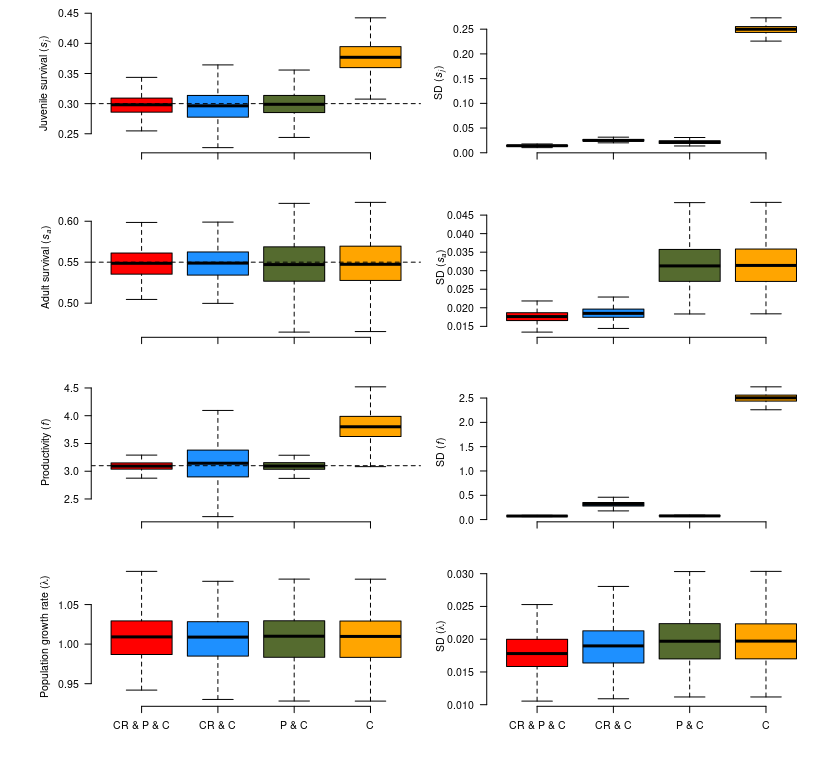
\includegraphics[width=17cm]{500sim_CountsJAD_28062022.png}
\caption{Boxplots des moyennes et des écart-types (SD) à posteriori de la survie des juvéniles ($s_j$) et des adultes ($s_a$), de la productivité($f$), et des taux de croissance de la population ($\lambda$) depuis quatre modèles démographiques différents utilisant différentes combinaisons de jeux de données : (1) IPM avec la capture-recapture, la productivité, et les données de comptage de la population dissociant la classe d'âge juvénile de celle des adultes ($CR \& P \& C$) ; (2) IPM avec la capture-recapture et les données de comptage de la population ($CR \& C$) ; (3)IPM avec la productivité et les données de comptage de la population dissociant la classe d'âge juvénile de celle des adultes ($P \& C$) ; et finalement (4) Un modèle démographique espace d'état avec les données de comptage de la population dissociant la classe d'âge juvénile de celle des adultes ($C$). Ces boxplots sont les résumés des moyennes à posteriori sur 500 simulations. La ligne horizontale en pointillés présente sur les trois premiers graphiques correspond aux valeurs du paramètre utilisées pour la simulation de données.}
\end{figure}

\end{document}

